\documentclass[animated,a4paper,slidestop,xcolor=pst,blue]{beamer}

\usepackage{beamerthemesplit}
\usepackage[utf8]{inputenc}
\usepackage[spanish]{babel}
\usepackage{graphicx}
\usepackage{pstricks} % PSTricks package
\usepackage{setspace}
\usepackage{multirow}
\usepackage{listings}
\usepackage{pgfpages}
\usepackage{hyperref}
\usepackage{etoolbox}
\usepackage{epstopdf}

\makeatletter
\patchcmd{\beamer@sectionintoc}{\vskip1.5em}{\vskip0.5em}{}{}
\makeatother

\setbeamercovered{dynamic}
\setcounter{tocdepth}{2}
\setbeamercolor{frametitle}{fg=black,bg=white}
\setbeamercolor{section in toc shaded}{fg=black}
\setbeamercolor{section in toc}{fg=red}
\setbeamercolor{subsection in toc shaded}{fg=black}
\setbeamercolor{subsection in toc}{fg=red}
\setbeamerfont{section in toc}{size=\small}
\setbeamerfont{subsection in toc}{size=\small}
\setbeamertemplate{section in toc shaded}[default][99]
\setbeamertemplate{subsection in toc shaded}[default][99]

\AtBeginSection[]
{\begin{frame}[c]
  \frametitle{Índice}
	\tableofcontents[currentsection,
        sectionstyle=show/shaded,
        subsectionstyle=hide]
\end{frame}}

\AtBeginSubsection[]
{\begin{frame}[c]
	\frametitle{Índice}
	\tableofcontents[
  		currentsection,
  		sectionstyle=shaded/shaded,
  		currentsubsection,
  		subsectionstyle=show/shaded/hide
		]
\end{frame}}

\setbeamercolor{frametitle}{fg=black,bg=white}

\setbeamertemplate{frametitle}{
	\begin{centering}
		\insertframetitle
		\par
	\end{centering}
}

\usetheme[secheader]{Boadilla}


\title[Diseño Sw]{Diseño Software}

\author[Pablo Sánchez]{\alert{Pablo Sánchez}}

\institute[I2E]{
		   Dpto. Ingenier{\'i}a Inform{\'a}tica y Electr{\'o}nica \\
		   Universidad de Cantabria \\
		   Santander (Cantabria, España) \\
		   p.sanchez@unican.es
}

\date{}

\begin{document}

\begin{frame}[c]
	\titlepage
	\begin{columns}
		\column{0.50\linewidth}
			\centering
    		
\includegraphics[width=.28\textwidth,keepaspectratio=true]{images/istr.eps}
		\column{0.50\linewidth}
			\centering
			
\includegraphics[width=.25\textwidth,keepaspectratio=true]{images/uc.eps}
	\end{columns}
\end{frame}

 \section{Introducción}

\begin{frame}[c]
	\frametitle{Profesorado}
	\begin{center}
		\alert{Pablo S\'{a}nchez Barreiro}  \\
		\begin{small}
		Despacho 1069 \\
		Departamento de Ingenier{\'i}a Inform{\'a}tica y Electr{\'o}nica \\
		p.sanchez@unican.es \\
		\end{small}
		\ \\
        \ \\
		Diego García Saiz  \\
		\begin{small}
		Despacho 1068 \\
		Departamento de Ingenier{\'i}a Inform{\'a}tica y Electr{\'o}nica \\
		diego.garcia@unican.es \\
		\end{small}
	\end{center}
\end{frame}

\begin{frame}[c]
	\frametitle{Horario Clases}
	\begin{small}
	\begin{center}
	\begin{tabular}{||l|c|c|c|c|c||}
	\hline \hline
				   & Lunes  & Martes  & Miércoles   & Jueves      & Viernes      \\ \hline \hline
    08:30 - 09:30  &        &         &             &             &              \\ \hline
	09:30 - 10:30  &        &         &             &             &              \\ \hline
	10:45 - 11:45  &        &         &             &             &              \\ \hline
	11:45 - 12:45  & Diseño & Diseño  & Diseño      &             &              \\ \hline
	12:45 - 13:45  &        &         & Diseño      &             &              \\ \hline \hline
	\end{tabular}
	\end{center}
	\end{small}
    \begin{enumerate}
        \item<2-> Para acudir a tutorías con los profesores se podrá hacer a cualquier hora, preferentemente en horario de mañana.
        \item<3-> Para asegurar la disponibilidad y atención al alumno, se recomienda avisar con antelación.
    \end{enumerate}
\end{frame}

\section{Objetivos y Temario}

\subsection{Objetivos}

\begin{frame}[c]
	\frametitle{Objetivos de la Asignatura}
	\begin{block}{Objetivos}
        Saber utilizar los principios, fundamentos, métodos, técnicas y herramientas para poder abordar satisfactoriamente las fases de \alert{diseño arquitectónico} y \alert{diseño detallado} de un proyecto software de mediana escala y perteneciente principalmente al dominio de los sistemas empresariales.
	\end{block}
\end{frame}

\begin{frame}[c]
	\frametitle{Objetivos de la Asignatura}
    \begin{center}
        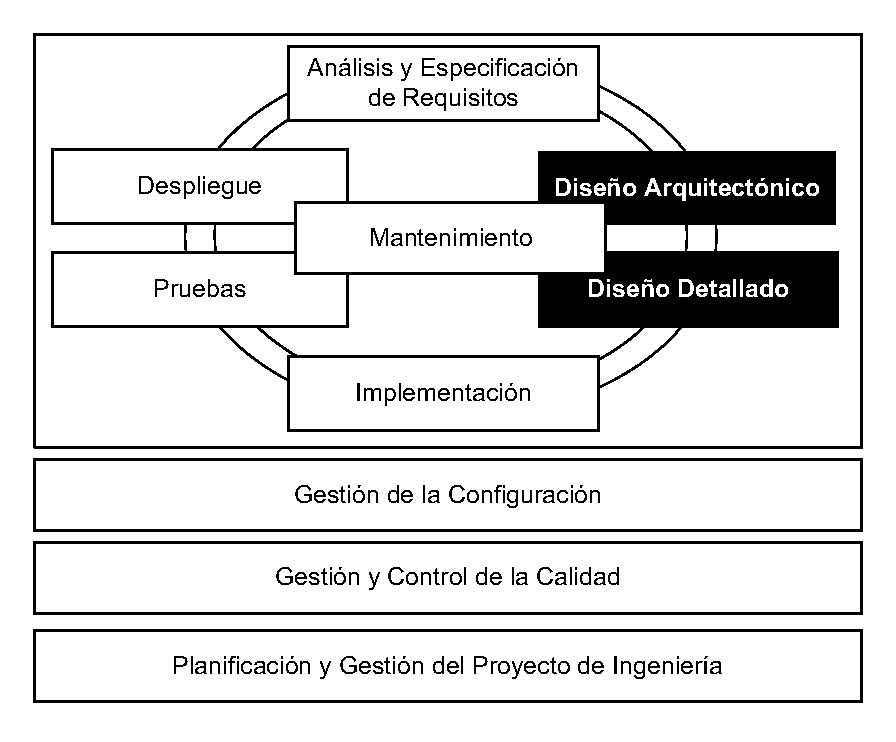
\includegraphics[width=0.75\linewidth,keepaspectratio=true]{images/cicloVida.eps}
    \end{center}
\end{frame}

\begin{frame}[c]
	\frametitle{Objetivos de Aprendizaje}
    \begin{enumerate}[<+->]
            \item Saber aplicar los principios \alert{GRASP} y \alert{SOLID}.
            \item Saber aplicar los principios de \alert{Diseño por Contrato}.
            \item Conocer y comprender la relación existente entre \alert{\emph{patrón de diseño}}, \alert{\emph{antipatrón}} y \alert{\emph{refactorización}}.
            \item Saber aplicar patrones de diseño microarquitectónicos, en especial, los \alert{patrones GoF}.
            \item Conocer y comprender algunos de los tipos principales de \alert{\emph{antipatrones}} existentes.
            \item Conocer y comprender algunos de los tipos principales de \alert{\emph{refactorizaciones}} existentes.
            \item Conocer y comprender el concepto de arquitectura sw.
            \item Saber aplicar patrones de diseño arquitectónicos, en especial los relativos a \alert{arquitecturas empresariales en tres capas}.
    \end{enumerate}
\end{frame}

\subsection{Temario}

\begin{frame}[c]
	\frametitle{Temario}
	\begin{enumerate}
		\item<1-> Principios Fundamentales del Diseño Software.
		\item<2-> Patrones de Diseño Software.
		\item<3-> Diseño e Implementación de Arquitecturas Software.
		\item<4-> Patrones Arquitectónicos para Arquitecturas Empresariales.
        \item<5-> Paradigmas de Programación No Orientados a Objetos.
	\end{enumerate}
\end{frame}

\section{Metodología}

\subsection{Plataforma}

\begin{frame}[c]
	\frametitle{Plataforma de Trabajo}
	\begin{itemize}
		\item<1-> La plataforma de trabajo será la asignatura es \emph{moodle}.
		\item<2-> Todas las notificaciones, publicaciones y entregas se harán a través de \emph{moodle}.
		\item<3-> \alert{Es obligación del alumno estar atento a las posibles notificaciones y avisos que se realicen a través de moodle}.
	\end{itemize}
\end{frame}

\subsection{Actividades}

\begin{frame}
	\frametitle{Clases de Aula}
	\begin{block}{Objetivo}
        Entender los conocimientos teóricos que constituyen la base de las habilidades y destrezas que se desarrollarán a lo largo de la asignatura.
	\end{block}
	\begin{itemize}
        \item<2-> Sin conocimiento teórico es imposible alcanzar las habilidades prácticas.
        \item<3-> La asistencia a las clases teóricas y prácticas no es obligatoria, \alert{pero si altamente recomendable e incluso necesaria}.
        \item<4-> La asignatura no está diseñada para ser seguida a distancia.
        \item<5-> Las clases serán fundamentalmente lecciones magistrales combinadas con alguna metodología activa.
        \item<6-> \alert{Las transparencias}, cuando las haya, \alert{no serán apuntes}.
        \item<7-> Todo tema tendrá asociado un itinerario para su aprendizaje de forma autónoma.
	\end{itemize}
\end{frame}

\begin{frame}[c]
	\frametitle{Clases de Laboratorio}
	\begin{block}{Objetivo}
        Aplicar los conceptos teóricos aprendidos en las clases de aula al desarrollo de un sistema software real de mediana escala, con el objetivo de desarrollar las competencias procedimentales y actitudinales deseadas.
	\end{block}
	\begin{itemize}
        \item<2-> Desarrollo de pequeñas prácticas individuales sobre problemas concretos.
        \item<3-> Se implementarán patrones de diseño en C\# y Java.
        \item<4-> No hay una receta única para hacer las prácticas, existen diferente soluciones alternativas posibles.
        \item<5-> Lo importante no es sólo que las prácticas funcionen, sino que los patrones que tratan de ejercitar se hayan aplicado correctamente.
	\end{itemize}
\end{frame}

\section{Métodos de Evaluación/Calificación}

\subsection{Fórmula Calificación}

\begin{frame}[c]
	\frametitle{Cálculo de la Calificación Final}
	\begin{block}{Fórmula de Cálculo de la Calificación Final}
		\begin{tabular}{lll}
			Calificacion Final  =  & PruebaPatrones     & $\times$ 0.50 + \\
                                   & PruebaArquitectura & $\times$ 0.50 + \\
                                   & TorreBabel         & $\times$ 0.10 \\
		\end{tabular}
	\end{block}
\end{frame}

\begin{frame}[c]
	\frametitle{Aclaraciones sobre la Evaluación}
	\begin{itemize}
        \item<2-> La prueba de patrones se celebrará a mediado o finales de Noviembre.
        %% 2O de Noviembre
        \item<3-> La prueba de arquitectura se celebrará en la convocatoria de exámenes de Enero.
        \item<5-> Una vez superada cualquiera de las pruebas, el alumno no tendrá que volver a realizarla dentro de ese curso académico.
        \item<5-> La prueba de patrones es recuperable en la convocatoria de Enero.
        \item<6-> Un alumno puede repetir una prueba si desea mejorar su calificación, pero en ese caso sólo computará la calificación de la última prueba realizada.
		\item<7-> Una calificación media de 4.99 es suspenso.
        \item<8-> La prueba opcional de la Torre de Babel puede servir para aprobar si se superan unos mínimos.
	\end{itemize}
\end{frame}

\subsection{Pruebas Evaluables}

\begin{frame}[c]
    \frametitle{Pruebas Evaluables}
	\begin{itemize}[<+->]
	   \item Las pruebas consistirán en pruebas prácticas de laboratorio que podrán contener además razonamientos sobre cuestiones teóricas.
       \item Se puede hacer uso en las pruebas de todo el material escrito o digital que se desee.
       \item El material escrito debe servir para consultar cuestiones puntuales, pero en el caso ideal no debería hacerse ningún uso del mismo.
       \item Se pueden preguntar durante las pruebas cuestiones relativas a la sintaxis de los lenguajes de programación o la utilización de sus librerías.
       \item Queda prohibido durante las pruebas el uso de dispositivos con capacidad de comunicación inalámbrica.
	\end{itemize}
\end{frame}

\subsection{Evaluación de las Prácticas}

\begin{frame}[c]
    \frametitle{Evaluación de las Prácticas}
	\begin{itemize}[<+->]
        \item<1-> No se realizarán entregas de prácticas semanales durante el curso.
        \item<2-> Como parte de las pruebas de laboratorio se podrá solicitar la entrega de una práctica o la realización de varias modificaciones sobre algunas de ellas.
        \item<3-> Las prácticas se pueden hacer en grupo, siempre y cuando se reconozca la autoría grupal.
        \item<4-> Se puede solicitar al profesor, y se recomienda hacerlo, una evaluación superficial de las prácticas antes de la realización de las pruebas evaluables.
    \end{itemize}
\end{frame}

\section{Bibliografía}

\begin{frame}[c]
	\frametitle{Bibliografía Principal}
    \begin{thebibliography}{1}

\bibitem{gamma:1994}
Erich Gamma, Richard Helm, Ralph Johnson, and John Vlissides.
\newblock {\em {Design Patterns: Elements of Reusable Object-Oriented
  Software}}.
\newblock Addison Wesley, November 1994.

\bibitem{Fowler2002}
Martin Fowler.
\newblock {\em {Patterns of Enterprise Application Architecture}}.
\newblock Addison-Wesley Professional, 2002.

\end{thebibliography}
\end{frame}

\begin{frame}[c]
	\frametitle{Bibliografía Secundaria}
    \begin{thebibliography}{1}

%\bibitem{felix:2008}
%F{\'e}lix~O. Garc{\'i}a, Javier Garz{\'a}s, Marcela~F. Genero, and Mario
%  Piattini.
%\newblock {\em {Medici{\'o}n y Estimaci{\'o}n del Software: T{\'e}cnicas y
%  M{\'e}todos para Mejorar la Calidad y la Productividad}}.
%\newblock Ra-Ma, 2008.

\bibitem{larman:2004}
Craig Larman.
\newblock {\em {Applying UML and Patterns: An Introduction to Object-Oriented
  Analysis and Design and Iterative Development}}.
\newblock Prentice Hall, 3 edition, OctoberPrentice 2004.

\bibitem{Martin2002}
Robert~C Martin.
\newblock {\em {Agile Software Development, Principles, Patterns, and
  Practices}}.
\newblock 2002.

\bibitem{meyer:2009}
Bertrand Meyer.
\newblock {\em {Touch of Class: Learning to Program Well with Objects and
  Contracts}}.
\newblock Springer, September 2009.


\end{thebibliography}
\end{frame}

\begin{frame}[c]
	\frametitle{Bibliografía Secundaria}
    \begin{thebibliography}{1}

%% Taylor

%\bibitem{felix:2008}
%F{\'e}lix~O. Garc{\'i}a, Javier Garz{\'a}s, Marcela~F. Genero, and Mario
%  Piattini.
%\newblock {\em {Medici{\'o}n y Estimaci{\'o}n del Software: T{\'e}cnicas y
%  M{\'e}todos para Mejorar la Calidad y la Productividad}}.
%\newblock Ra-Ma, 2008.

\bibitem{Freeman2004}
Erick Freeman, Elisabeth Robson, Bert Bate, and Kathy Sierra.
\newblock {\em {Head First Design Patterns}}.
\newblock O'Reilly, 2004.

\bibitem{brown:1998}
William J. Brown, Raphael C. Malveau, Hays W. ``Skip'' McCormick, and Thomas J. Mowbray,
\newblock {\em {AntiPatterns: Refactoring Software, Architectures and Projects in Crisis}}
\newblock Wiley, 1998.


\end{thebibliography}
\end{frame}

\end{document}
